\documentclass[border=4pt]{standalone}
\usepackage{amsmath,amssymb}
\usepackage{tikz}
\usetikzlibrary{arrows.meta,shadows,calc}
\begin{document}
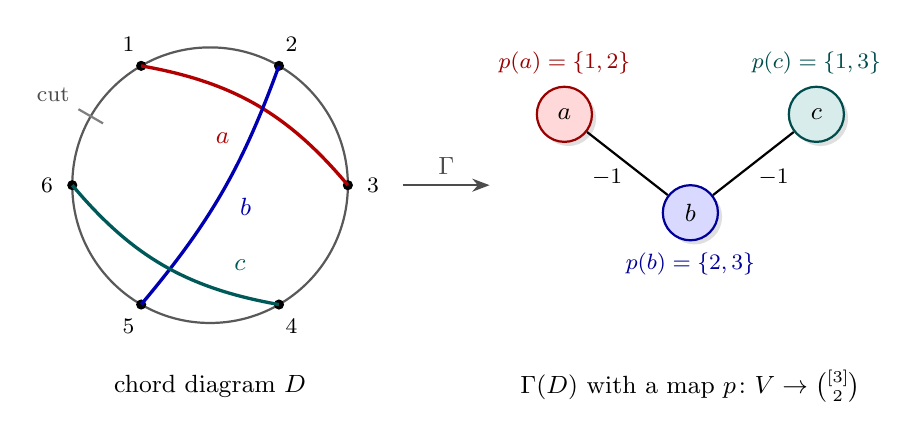
\begin{tikzpicture}[
  pt/.style={circle,fill=black,inner sep=1.3pt},
  vx/.style={circle,draw=#1!60!black,fill=#1!15,thick,minimum size=7mm,font=\small,
             drop shadow={opacity=0.25,shadow xshift=1.5pt,shadow yshift=-1.5pt}},
  lab/.style={font=\footnotesize,fill=white,inner sep=1.5pt,rounded corners=1pt},
  >={Stealth[length=2.2mm]}]
  % chord diagram: points 1..6 on the circle, cut between 6 and 1
  \def\R{1.75}
  \draw[thick,gray!70!black] (0,0) circle (\R);
  \foreach \k in {1,...,6} {
    \coordinate (P\k) at ({120-60*(\k-1)}:\R);
    \node[pt] at (P\k) {};
    \node[font=\footnotesize] at ({120-60*(\k-1)}:{\R+0.32}) {$\k$};
  }
  \draw[very thick,red!70!black]  (P1) to[bend left=20] (P3);
  \draw[very thick,blue!70!black] (P2) to[bend left=10] (P5);
  \draw[very thick,teal!70!black] (P4) to[bend left=20] (P6);
  \draw[thick,gray] ({150}:{\R-0.18}) -- ({150}:{\R+0.18});
  \node[font=\footnotesize,gray!60!black] at (150:{\R+0.55}) {cut};
  \node[font=\small,red!70!black]  at (75:0.62) {$a$};
  \node[font=\small,blue!70!black] at (0.45,-0.28) {$b$};
  \node[font=\small,teal!70!black] at (0.38,-1.02) {$c$};
  \node[font=\small] at (0,-2.55) {chord diagram $D$};
  % arrow
  \draw[->,thick,gray!60!black] (2.45,0) -- node[above,font=\small]{$\Gamma$} (3.55,0);
  % intersection graph with an assignment p
  \begin{scope}[xshift=6.1cm]
    \node[vx=red]  (a) at (-1.6,0.9) {$a$};
    \node[vx=blue] (b) at (0,-0.35) {$b$};
    \node[vx=teal] (c) at (1.6,0.9) {$c$};
    \draw[thick] (a) -- node[lab,below left]{$-1$} (b);
    \draw[thick] (b) -- node[lab,below right]{$-1$} (c);
    \node[font=\footnotesize,red!60!black]  at (-1.6,1.55) {$p(a)=\{1,2\}$};
    \node[font=\footnotesize,blue!60!black] at (0,-1.0) {$p(b)=\{2,3\}$};
    \node[font=\footnotesize,teal!60!black] at (1.6,1.55) {$p(c)=\{1,3\}$};
    \node[font=\small] at (0,-2.55) {$\Gamma(D)$ with a map $p\colon V\to\binom{[3]}{2}$};
  \end{scope}
\end{tikzpicture}
\end{document}
